\documentclass{article}
\usepackage[utf8]{inputenc}
\usepackage{amsmath}
\usepackage{listings}
\usepackage{geometry}
\usepackage{graphicx}
\usepackage{appendix}
\usepackage{subfig}
\usepackage{gensymb}
\usepackage{cancel}
\usepackage{physics}
\usepackage{empheq}
\usepackage{wrapfig}
\usepackage[colorlinks=true]{hyperref}
\usepackage{xcolor}
\usepackage{geometry}
\geometry{bottom=20mm}
\definecolor{codegreen}{rgb}{0,0.6,0}
\definecolor{codegray}{rgb}{0.5,0.5,0.5}
\definecolor{codepurple}{rgb}{0.58,0,0.82}
\definecolor{backcolour}{rgb}{0.95,0.95,0.92}
\lstdefinestyle{mystyle}{
    backgroundcolor=\color{backcolour},   
    commentstyle=\color{codegreen},
    keywordstyle=\color{magenta},
    numberstyle=\tiny\color{codegray},
    stringstyle=\color{codepurple},
    basicstyle=\ttfamily\footnotesize,
    breakatwhitespace=false,         
    breaklines=true,                 
    captionpos=b,                    
    keepspaces=true,                 
    numbers=left,                    
    numbersep=5pt,                  
    showspaces=false,                
    showstringspaces=false,
    showtabs=false,                  
    tabsize=2
}

\lstset{style=mystyle}

\title{%
Mandatory Assignment 2 \\
\large STK-IN4300}
\author{Simen Løken}
\date{November 2022}

\begin{document}

\maketitle
\renewcommand{\thesection}{Problem \arabic{section}}
\renewcommand{\thesubsection}{\arabic{subsection})}
\section{Regression}
\subsection{}
We dichotomize and use a $1/3$ $2/3$ \texttt{test}/\texttt{train} split, plotting the observed \texttt{LC50} against the predicted \texttt{LC50}:
\begin{figure}[ht!]
    \centering
    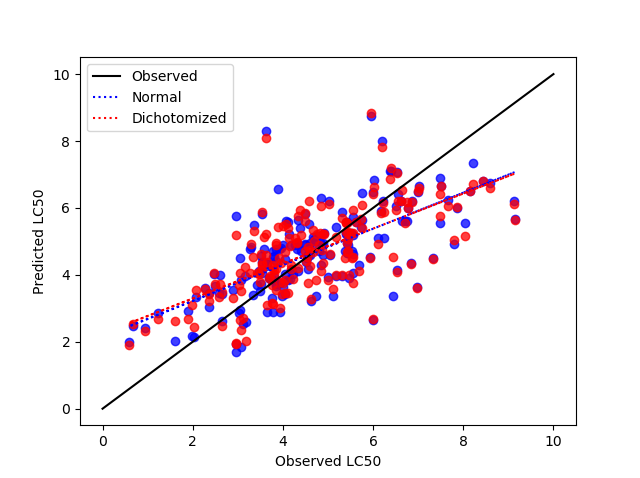
\includegraphics[scale=0.5]{regression1.png}
    \caption{A scatter plot of our predicted values on the y-axis against their observed values on the x-axis. Ideally any values should lie alongside the "observed" or nominal line in black.}
    \label{figR1}
\end{figure} \newline
As we can see, an undichotomized dataset outperforms its dichotomized counterpart just barely (the blue dashed line is close to the nominal black than the red). \newline As for the test error, we get:
\begin{equation*}
    \texttt{MAE} = 0.9172
\end{equation*}
\begin{equation*}
    \texttt{MAE}_d = 0.9366
\end{equation*}
where the $_d$ signifies the dichotomized error. This tells us that what we already know from Figure [\ref{figR1}], namely that our non-dichotomized model performs better than its counterpart. \newpage
Additionally, we retrieve the following regression coefficients:
\begin{table}[ht!]
    \centering
    \begin{tabular}{c|c|c|}
         &Normal& Dichotomized \\
         \hline
         \texttt{TPSA}& 1.3635& 1.1205 \\
         \texttt{SAacc}&-1.0259& -0.8218 \\
         \texttt{H050}&0.0694& -0.0734 \\
         \texttt{ML0GP}&0.7921& 0.8614 \\
         \texttt{RDCHI}&0.4530& 0.3298 \\
         \texttt{GATS1p}&-0.2054& -0.1796 \\
         \texttt{nN}&-0.4049& 0.0116 \\
        \texttt{C040}& -0.0083& -0.0745 \\

    \end{tabular}
    \caption{A table showing our regression coefficients}
    \label{tabR1}
\end{table} \newline
We see here that, generally, the regression coefficients for the dichotomized model are weaker than their normal counterparts, which is likely what causes the worse fit.
\subsection{}
We get:
\begin{figure}[ht!]
    \centering
    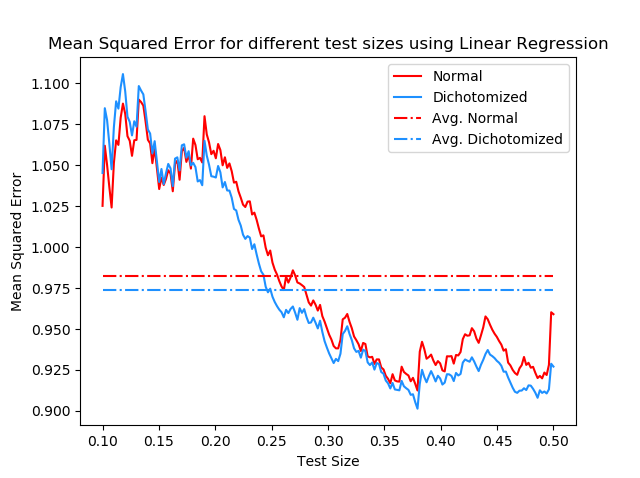
\includegraphics[scale=0.5]{regression2.png}
    \caption{A figure showing the Mean Absolute Error (MAE) for different test sizes of our normal and dichotomized model, plus their average.}
    \label{figR2}
\end{figure} \newline
which is actually the opposite of what I (and seemingly the sub problem) was expecting. As to why this is the case, I cannot say, it could simply come down to "bad luck" given the random nature of fitting models, but I can explain why a model is \emph{usually} worsened by dichotomizing variables.
\newline
The most obvious one is losing "resolution", and by extension information whenever we dichotomize an array. What we're doing, in layman's terms, is postulating that to the model it should only matter \emph{if} there are any hydrogen atoms bonded to heteroatoms, nitrogen in the molocule etc... The amount is irrelevant. \newline
Given that the numbers we've dichotomized for some cases reach all the way up into the 10s, it is hard to justify dichotomizing our data. Perhaps quantizing would be better, at given thresholds. \newline
As it stands now, the result in Figure [\ref{figR2}] tells us that the number of the respective atoms do not matter, it only matters that the respective atoms are present.
\subsection{}
We examine the the model using stopping criterion and feature selection, and look at $R^2$ scores. We get 4 features selected, the same for backward and forward, and those are: \texttt{TPSA, SAacc, ML0GP, GATS1p}. This is, from what I understand, rather uncommon, and only happens after tuning the alpha hyperparameter of \texttt{Lasso}, which was necessary in this case as not tuning it resulted in negative $R^2$ values for feature selected fits.
\newline We get the following $R^2$ values:
\begin{equation*}
    \begin{gathered}
        R^2_{AIC} = 0.452 \;\;\; R^2_{BIC} = 0.459 \\ R^2_{F} = R^2_B = 0.447
    \end{gathered}
\end{equation*}
$R^2_F$ and $R^2_B$ are of course equal because both forward and backward selection chose the same four variables. 
\subsection{}
We choose to look at the alpha regularization hyperparameter of Ridge Regression. We let it go from \texttt{0.1} to \texttt{12}, giving us the following result:
\begin{figure}[ht!]
    \centering
    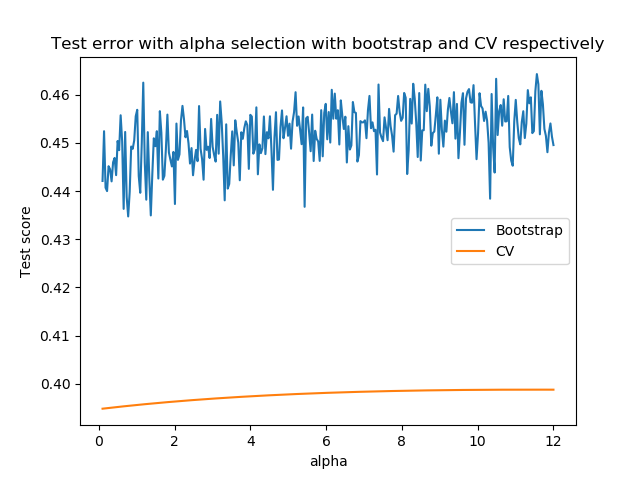
\includegraphics[scale=0.5]{regression3.png}
    \caption{A figure showing how test score varies with alpha selection \newline It's worth mentioning that this is not using deviance as requested in the assignment text, as I couldn't get a deviance scorer to work for both methods.}
    \label{figR3}
\end{figure} \newline
The most interesting result here is the variance in the smoothness of the test scores. Whereas the test score for the bootstrap method is strictly better than cross-validation, cross-validation is a lot smoother and more stable. This makes sense when you think about the way cross validation works and how we find the mean of $x$-folds. You're less likely to have dramatic "jumps" in test scores.
\newpage
\subsection{}
We use three different smoothing splines in:
\begin{table}[ht!]
    \centering
    \begin{tabular}{c|c}
         Spline& MAE \\
         \hline
         \texttt{SAacc}, \texttt{ML0GP}& 0.89 \\
         \texttt{nN}, \texttt{H050}& 1.12 \\
         \texttt{GATS1p}, \texttt{SAacc}& 0.97 \\
         \hline
    \end{tabular}
    \caption{Mean Absolute Error for three different splines using a GAM approach. \newline
    Refer to the assignment text \cite{assign} for spline variable definitions}
    \label{tabR2}
\end{table} \newline
We see that we get less than satisfactory results, with mean absolute errors around 1. Additionally, we see that for low variance, low resolution variables like the \texttt{nN}, \texttt{H050} spline, we get poorer results than with the other splines. This lends further credence to the features selected by forward selection/backward elimination in task 3, in that these variables are less statistically important than the others. You could also argue this could be one of the reasons as to why we saw better performance with these variables dichotomized in 2).
\subsection{}
We get the following tree:
\begin{figure}[ht!]
    \centering
    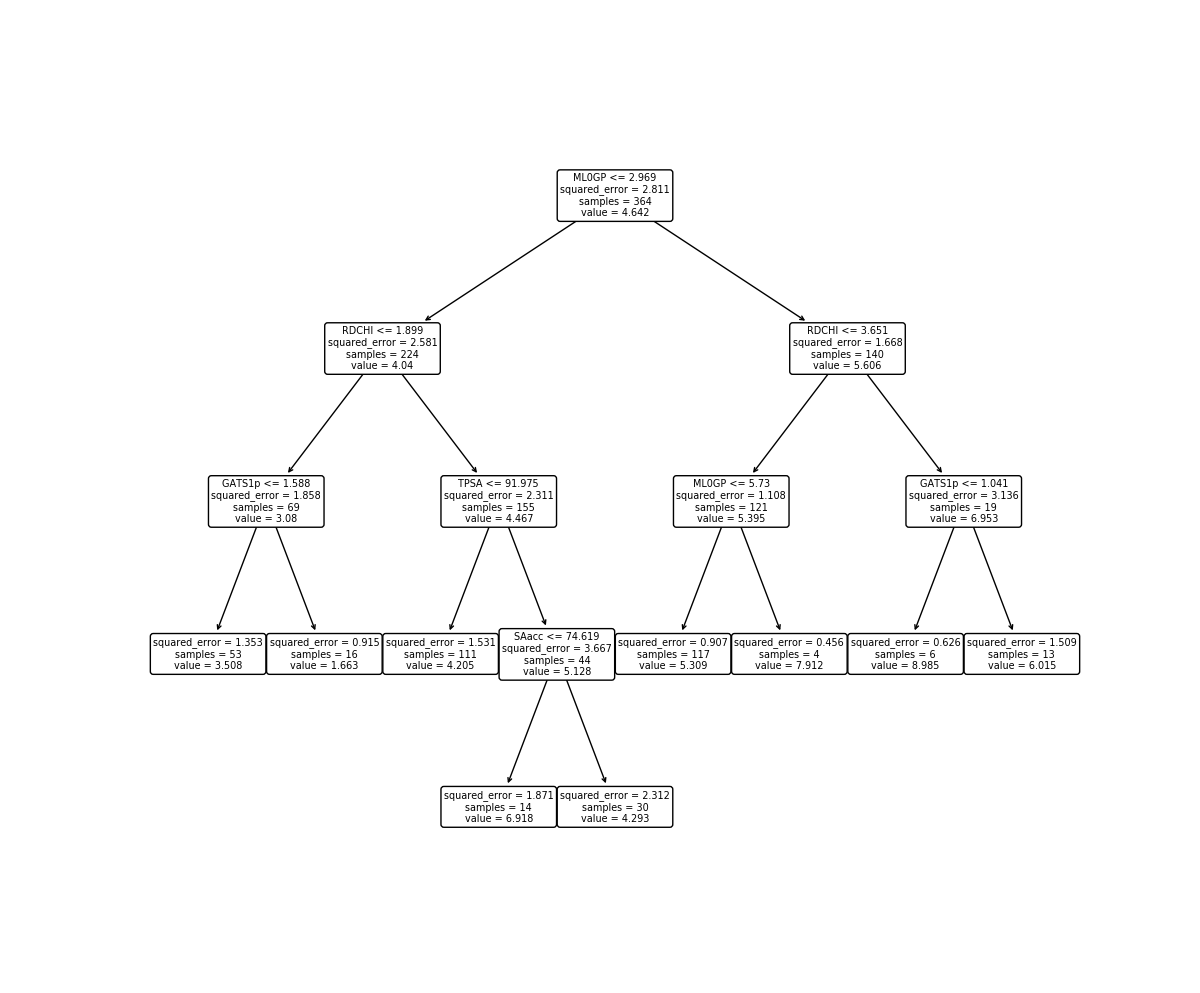
\includegraphics[scale=0.4]{regression4.png}
    \caption{Our tree. Modeled such that, for example at the "root" node, if \texttt{ML0GP} $\leq$ 2.969, go left, if not go right}
    \label{figR4}
\end{figure} \newline
As for how we decided this model, we use a tuning parameter alpha which controls how much of the tree we prune to prevent overfitting the model. We simply use the \texttt{cost\_complexity\_pruning\_path} method in \texttt{scikit-learn} to get a range of possible alpha parameters, before finding the one that provides the best test score. \newpage Additionally, we can examine how the tree is pruned as we increase alpha:
\begin{figure}[ht!]
    \centering
    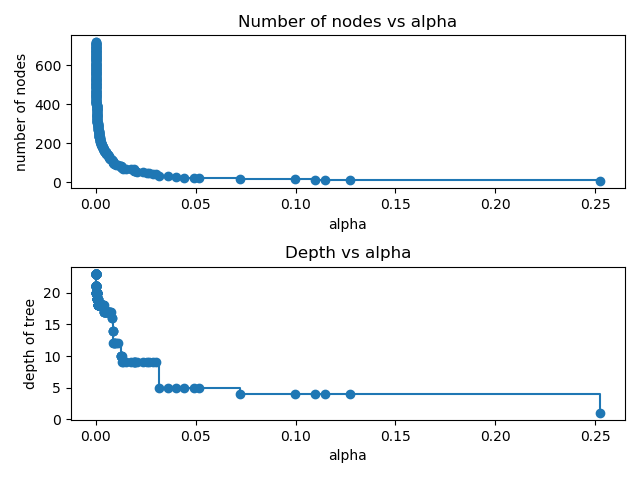
\includegraphics[scale=0.5]{regression5.png}
    \caption{Showing how the depth and total number of nodes of the tree decreases as we increase alpha. In our case the sweetspot is at just over 0.05}
    \label{figR5}
\end{figure} \newline

\subsection{}
Lastly, let us look at the test and training error of all our methods:
\begin{table}[ht!]
    \centering
    \begin{tabular}{c|c|c}
         & Train Error [MAE] & Test Error [MAE]  \\
         \hline
         1)&  \\
         Normal & 0.92 & 0.90 \\
         Dichotomized& 0.94& 0.94 \\ 
         3)& \\
         AIC&  0.2& 0.81 \\
         BIC& 0.22&  0.79\\
         FORWARD& 0.40& 0.66 \\
         BACKWARD& 0.40& 0.66 \\
         4)& \\
         BOOTSTRAP& 0.92& 0.93 \\
         CV& 0.91& 0.95 \\
         5)& \\
         GAM& & 0.89 \\
         6)& \\
         TREE& 0.94& 0.85
    \end{tabular}
    \caption{All test and train errors for our models in Mean Absolute Error. \newline
    Note that the training error for GAM is missing as I couldn't find a way to retrieve it.}
    \label{tabErrs}
\end{table} \newline
We see that most of the models are pretty bad, most likely because of lack of tuning. However, the greatest performer (by a large margin) is the forward selection/backward elimination solution. This is likely because forward selection/backward elimination is a "parameter" in itself, that is, this model is not "raw" in the same sense that the other models are.
\newpage
\section{Classification}
\subsection{}
We run the code and find the following plot:
\begin{figure}[ht!]
    \centering
    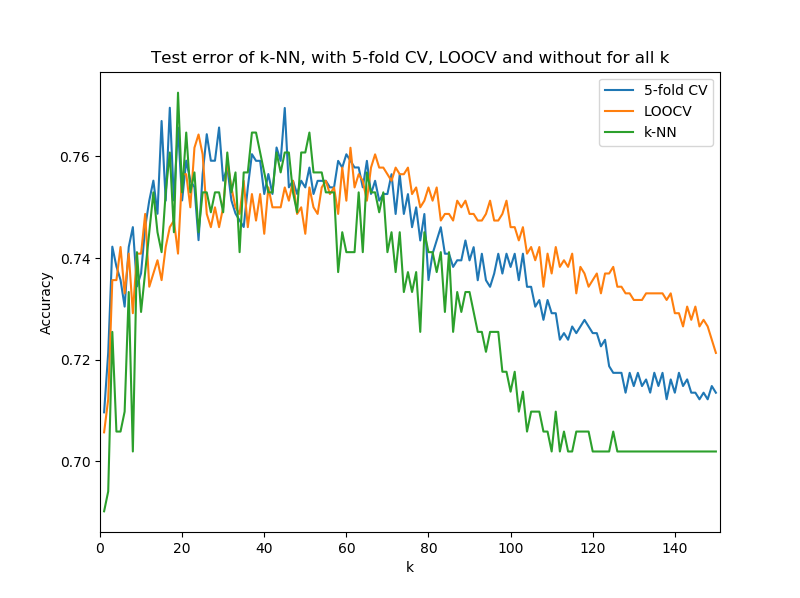
\includegraphics[scale=0.5]{classification1.png}
    \caption{A figure showing the accuracy for all possible $k$ using three different methods.}
    \label{figC1}
\end{figure} \newline
What's interesting here to me is that the pure \texttt{k-NN} actually achieves a higher accuracy than the 5-fold or leave one out cross-validation methods for select small $k$. For most other $k$ however, \texttt{k-NN} is outperformed by the cross-validation methods. As to why \texttt{k-NN} outperforms the cross-validation methods at certain $k$s, this could just come down to statistical luck, given the random nature.
\newpage
\subsection{} 
We use a GAM method to examine a given variables effect on the response:
\begin{figure}[ht!]
    \centering
    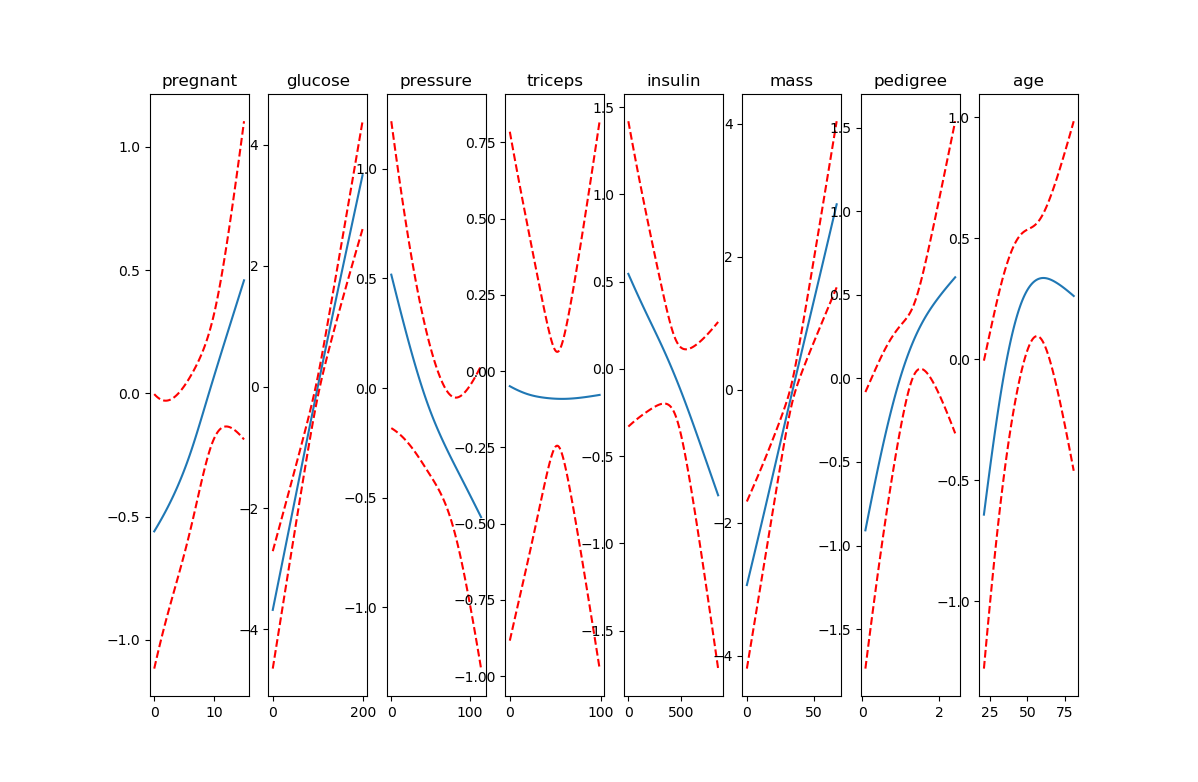
\includegraphics[scale=0.35]{classification2.png}
    \caption{A figure showing how much a variable corresponds with either a positive/negative diabetes classification. The dotted red lines are the uncertainties. Overall accuracy score: 0.77}
    \label{figC2}
\end{figure} \newline
Unsurprisingly, we see here a very clear correlation between glucose levels, insulin leves, blood pressure and mass, four variables all very commonly associated with diabetes. Additionally, we can also see clearly that women who've not been pregnant trend towards a negative response. The same goes for age, where younger women are less likely to have diabetes. The only variable which seemingly has very little to no correlation with diabetes is the triceps (skin fold thickness), at least for this particular model. Perhaps we could consider culling this variable entirely from our data.
\subsection{}
We then find:
\begin{table}[ht!]
    \centering
    \begin{tabular}{c|c|c}
         & \texttt{Train} & \texttt{Test} \\
         \hline
         \texttt{DT}&  1.0& 0.72 \\
         \texttt{PR}& 0.99& 0.75 \\
         \texttt{CO}& 0.99& 0.77 \\
         \texttt{RF}& 1.0& 0.79 \\
         \texttt{AB}& 0.84& 0.76 \\
    \end{tabular}
    \caption{A table showing the training and test error for different ensemble methods \newline \textit{\texttt{DT}: Decision Tree, \texttt{PR}: Bagging w/ Probability voting, \texttt{CO}: Bagging w/ Consensus voting, \texttt{RF}: Random Forest, \texttt{AB}: AdaBoost}}
    \label{tabC1}
\end{table} \newline
We notice that the train error is generally high for all but AdaBoost. This is often indicative of overfitting, which could explain our test scores generally plateauing in the mid-70s, and suggests to us that all models but the AdaBoost model is overfitted. Luckily this doesn't have too much of an effect on our test scores (at least relatively to the not-so-overfitted AdaBoost) \newpage
\subsection{}
As it stands right now, with just these results and no extra tinkering/tuning I'd say GAM has the most raw analyzing power. In my opinion, I find GAM to be the easiest in terms of reading off which variables matter the most for a given set of data. This in turn of course makes analyzes easier. Of course, that doesn't necessarily make it the best model. There's a case to be made for \texttt{k-NN} too, which is a very strong classifier all things considered. Generally most methods are about equal accuracy-wise, although they could likely be substantially improved if I took the time to sufficiently tune parameters. As for the 5 models just above, they're all very overfitted, but this too could in all likelihood be fixed if time was taken to tune parameters.
\subsection{}
Let us now examine new results with corrected data:
\newline The updated Figure [\ref{figC1}]:
\begin{figure}[ht!]
    \centering
    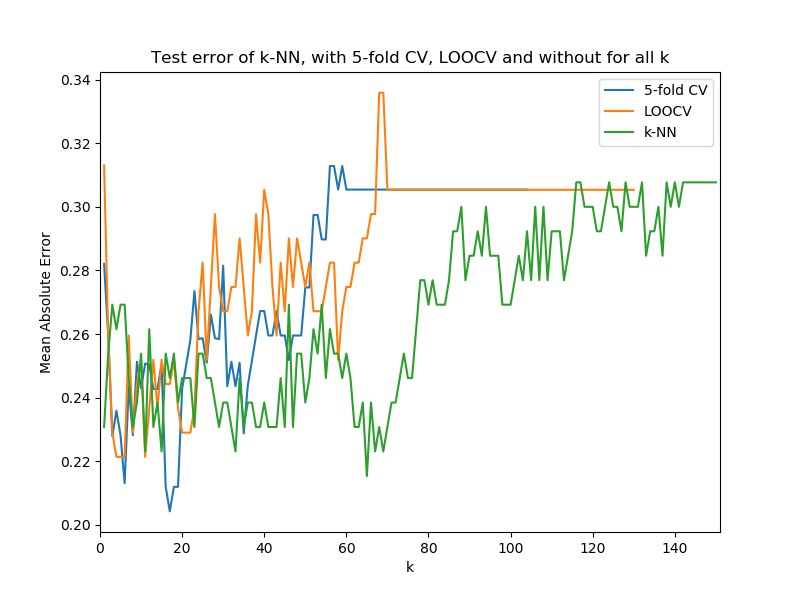
\includegraphics[scale=0.5]{classification1corrected.png}
    \caption{A figure showing the accuracy for all possible $k$ using three different methods.}
    \label{figC3}
\end{figure} \newline
Again we find that \texttt{k-NN} outperforms the other methods early, but then rapidly falls off again. Else we see that the accuracy is higher than in Figure [\ref{figC1}], indicating that the false/wrong data "poisoning" was having a significant effect on our model. It is also worth noting that this model is a lot more stable for different $k$ than our previous model. 
\newpage Let us now examine our GAM results:
\begin{figure}[ht!]
    \centering
    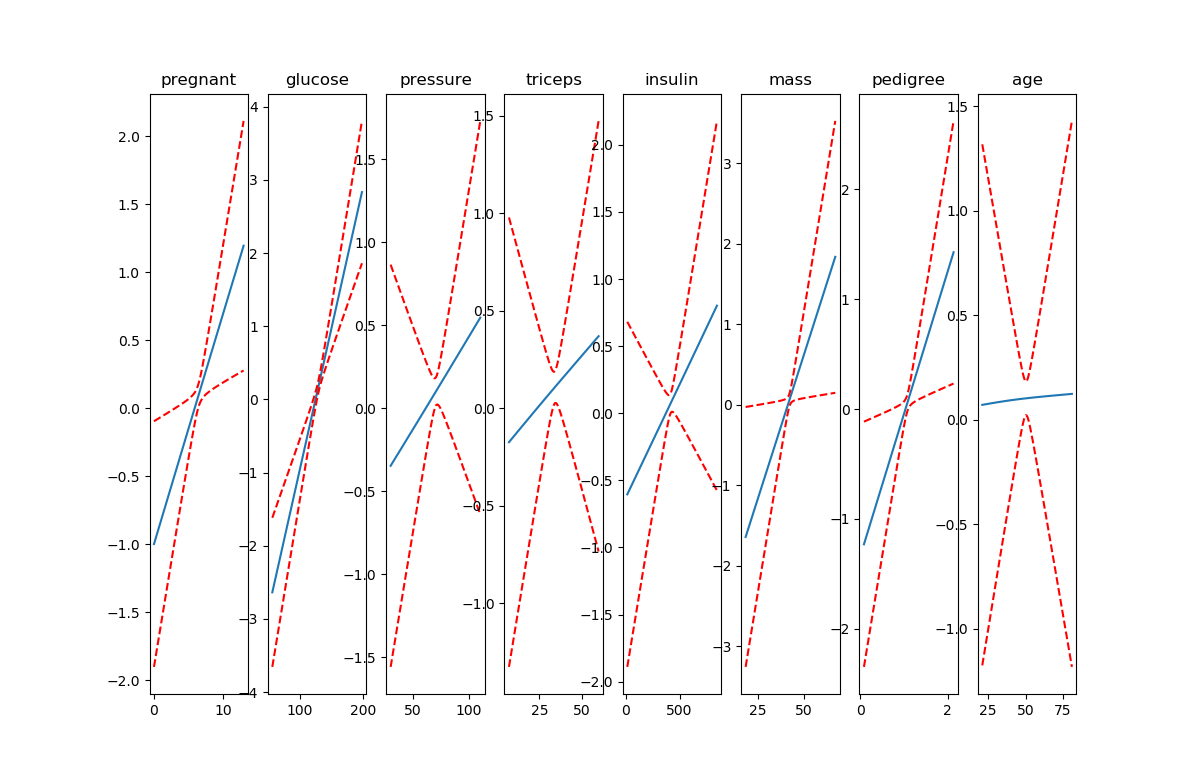
\includegraphics[scale=0.35]{classification2corrected.png}
    \caption{A figure showing how much a variable corresponds with either a positive/negative diabetes classification. The dotted red lines are the uncertainties. Overall accuracy score: 0.77}
    \label{figC4}
\end{figure} \newline
We see now that our results have changed somewhat. While we now have a lot more clear correlations (notice all the linear relations), we also now have a lot more uncertainty regarding each correlation, except for  glucose. We see also now that triceps (which we considered culling from the data in Figure [\ref{figC2}] now has a linear relation with diabetes. However, we also see that according to this model high insulin corresponds with diabetes, which is opposite of what we see in reality, where diabetics produce little to no insulin (and thus have high glucose, as seen here).
\newline
Lastly the table now becomes
\begin{table}[ht!]
    \centering
    \begin{tabular}{c|c|c}
         & \texttt{Train} & \texttt{Test} \\
         \hline
         \texttt{DT}&  1.0& 0.77 \\
         \texttt{PR}& 0.98& 0.79 \\
         \texttt{CO}& 0.97& 0.76 \\
         \texttt{RF}& 1.0& 0.79 \\
         \texttt{AB}& 0.95& 0.77 \\
    \end{tabular}
    \caption{A table showing the training and test error for different ensemble methods \newline \textit{\texttt{DT}: Decision Tree, \texttt{PR}: Bagging w/ Probability voting, \texttt{CO}: Bagging w/ Consensus voting, \texttt{RF}: Random Forest, \texttt{AB}: AdaBoost}}
    \label{tabC1}
\end{table} \newline
Generally, the train error has had little to no changes whereas we see an improved performance for all test scores but bagging with consensus voting and random forest. The overfitting issue is still not fixed, sadly, and has actually worsened for AdaBoost. Again, we could very likely fix this by applying stricter penalization parameters and general tuning.
\bibliographystyle{unsrturl}
\bibliography{citations.bib}
\newpage
\section*{Appendix - Code}
Given the length of the code I thought it'd be nicer to link to a github reposity instead. \newline
The code can be found at \url{https://github.com/simloken/STK-IN4300/tree/master/Assignment_2}
\end{document}
